\section{Âmbito do Produto}
\subsection{Fronteira do Produto}
\begin{figure}[!htb]
	\centering
	\includegraphics[scale=0.85]{images/diagramaGeralDeUseCase}
	\caption {Diagrama geral de \emph{Use Cases} do produto}
\end{figure}

\subsection{Use Case Individuais do Produto}
\subsubsection{\textbf{1 - Realizar Simulação de Seguro Automóvel}}
Qualquer utilizador do produto poderá efectuar uma simulação de seguro automóvel. No entanto, cada utlizador terá acesso a pequenas funcionalidades diferentes dependendo do tipo de utiliador em que se insere (registado ou não, mediador, etc). Aqui apresentaremos o fluxo normal deste \emph{use case} para um utilizador básico, ou seja, sem qualquer tipo de privilégios. Mais à frente, na explicação dos \emph{use cases} que se seguem, abordaremos as funcionalidades extra que cada tipo de utilizador terá. 
\begin{figure}[!htb]
	\centering
	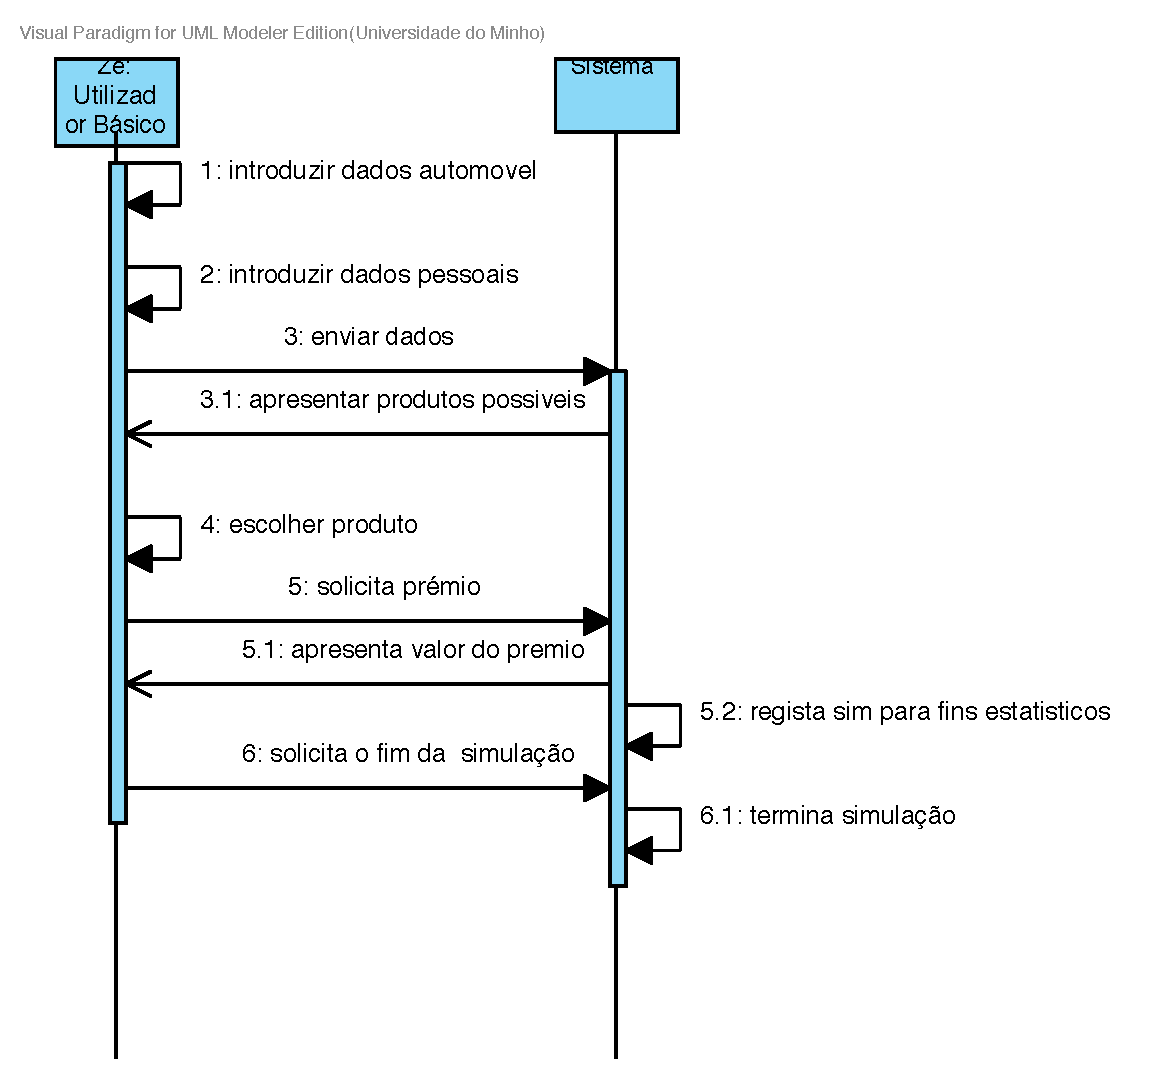
\includegraphics[scale=0.70]{images/simAuto}
	\caption {Diagrama de fluxo de uma simulação automóvel}
\end{figure}
\pagebreak

\noindent Este diagrama tenta abstrair de forma informal a sequência básica que será seguida de modo a efectuar uma simulação automóvel. 

Os dados automóvel mencionados no passo (1) que estamos a considerar relevantes para efectuar uma simulação são os seguintes: data de construção, marca, modelo, versão do modelo, cilindrada, potência e número de portas do automóvel. 

Quanto aos dados do condutor, estes são: data de nascimento, sexo, código postal da área de residência do condutor, número de acidentes nos últimos cinco anos em que o condutor foi dado como culpado, se a presente simulação se refere ao primeiro seguro automóvel e data de início de novo seguro. 

Com base nos dados nos dados introduzidos o sistema apresenta os produtos passíveis de serem escolhidos pelo utilizador, sendo que pode escolher um leque de coberturas dentro de cada produto. A fórmula que estamos a considerar actualmente para cálculo do prémio é a seguinte:

Prémio comercial = valor base produto * ponderador marca/modelo (tipo, cilindrada e potência) * ponderador extras veículo * ponderador idade condutor * ponderador zona circulação * ponderador ramo laboral * ponderador tipo pagamento * ponderador sexo

Bónus/Malus = pontuação experiência condução + pontuação número de acidentes + desconto
OU
Bónus/Malus = transferência do seguro anterior

Prémio total = Prémio comercial + Bónus/Malus + Taxas(apólice, carta verde, inem, fundap/fga, selo apólice)

\subsubsection{\textbf{2 - Realizar Simulação de Seguro de Saúde}}
A realização de seguro de saúde é semelhante à automóvel, sendo que os dados a serem fornecidos são diferentes. De momento, estamos a considerar relevantes apenas o sexo e data de nascimento das pessoas seguradas, assim como o grau de parentesco entre si. Temos portanto em conta que podem ser seguradas várias pessoas e que o tomador não é necessariamente uma delas.

\subsubsection{\textbf{3 - Realizar Simulação Multi-Produto}}
É possível incluir vários produtos numa mesma simulação. Para o efeito, o utilizador procederá como numa simulação normal, preenchendo os dados correspondentes ao primeiro produto a simular. Terminada esta simulação, é apresentada ao utilizador a opção "acrescentar novo produto (simulação multi-produto)" que, quando seleccionada, agrega a presente simulação à carteira de simulações e apresenta a possibilidade de realização de simulação de um novo produto. 

Repetindo este processo, e quando satisfeito com o número de produtos simulados, o Utilizador solicita o cálculo do prémio conjunto, que tem em conta os descontos aplicáveis a uma simulação multi-produto.

\subsubsection{\textbf{4 - Pesquisar e Consultar Simulações}}
A cada utilizador registado com simulações guardadas será dada a possibilidade de pesquisar pelas mesmas. Tal significa filtrar as simulações guardadas por produto, valor do prémio, etc. O mediador poderá também pesquisar as simulações dos seus clientes. O sistema permite também a consulta das simulações pesquisadas.

\subsubsection{\textbf{21(auto), 22(saúde),23(multi) - Gerir Simulações}}
Um mediador poderá lançar novas simulações para a 
área de notificação de um cliente seu. Terá, para esse fim, de aceder ao cliente desejado a partir da sua carteira de clientes e efectuar a simulação referida. No fim, terá a hipótese de a enviar para área de notificação desse cliente.

\subsubsection{\textbf{5 - Rescindir Apólice}}
O mediador terá permissões para anular uma apólice existente. Para tal, terá de aceder, na ficha dos seus clientes, ao cliente que solicitou o término da mesma e solicitar a anulação da mesma.

\subsubsection{\textbf{6 - Alterar Apólice}}
O mediador tem permissão também para modificar um contrato existente. Segue um fluxo semelhante à tarefa de anular uma apólice.

\subsubsection{\textbf{7 - Pedir Estatísticas}}
O administrador do sistema poderá pedir ao sistema as estatísticas relativas às simulações efectuadas.  Ser-lhe-á possível discriminar o tipo de valores estatísticos que pretende. Por exemplo, referentes apenas a simulações efectuadas por utilizadores não registados, registados ou ambos. Para cada um deles serão apresentados os valores referentes ao número de simulações por produto e por período, valor total dos prémios por produto e por período, entre outros a definir posteriormente.

\subsubsection{\textbf{8 - Configurar Descontos}}
O Colaborador será capaz de introduzir ou configurar no sistema novos descontos. Sejam eles promoções temporais (promoção de Natal por exemplo) ou descontos aplicados à compra de seguros multi-produto. A configuração de descontos permitirá também atribuir valores de desconto diferentes a diferentes tipos de mediadores clientes dependendo do seu mérito ou rentabilidade, respectivamente. 

\subsubsection{\textbf{9 - Registar Simulação}}
Será permitido a todos os utilizadores registados gravar uma simulação efectuada no seu histórico de simulações. Bastando para isso que tal o indique no fim de uma simulação. O sistema encarregar-se-á de guardar todos os dados numa base de dados, estando depois a mesma  disponível ao cliente para consulta e modificação.

\subsubsection{\textbf{10 - Apagar Simulações}}
Será também possível apagar uma simulação anteriormente gravada. Tudo o que o utilizador precisará de fazer é aceder à mesma, como se de uma consulta normal se tratasse e solicitar ao sistema a remoção da mesma do seu histórico de simulações, possivelmente através de apenas um clique num botão.

\subsubsection{\textbf{15 - Passar Simulação a Contrato}}
Tanto um cliente como um mediador poderão preencher um contrato online. Após uma simulação estar terminada, será dada a opção de concretizar essa simulação passando-a a contrato, caso em que apenas terão de ser preenchidos adicionalmente alguns dados pessoais do cliente e/ou outros que forem necessários. O esquema seguinte visa representar o fluxo desta operação:
\pagebreak
\begin{figure}[!htb]
	\centering
	\includegraphics[scale=0.75]{images/efectuarContrato}
	\caption {Diagrama de fluxo da operação de passar uma simulação a contrato}
\end{figure}

\subsubsection{\textbf{17 - Imprimir Contrato}}
Um cliente pode a partir de sua casa efectuar uma simulação e passa-la a contrato (que terá depois que ser validado por um mediador). Esse contrato consiste na colecção de dados necessários ao mesmo e é passível de ser impresso. Para tal, o utilizador necessita apenas de, depois de efectuada a simulação e preenchidos os campos obrigatórios do contrato, solicitar a impressão do documento ao sistema.

\subsubsection{\textbf{17 - Imprimir Apólice}}
Após um contrato estar formalizado no sistema, o mediador terá a possibilidade de imprimir a apólice correspondente após ter validado o mesmo.

\subsubsection{\textbf{19 - Validar Contrato}}
Qualquer utilizador resgistado pode passar uma simulação a contrato. No entanto, nenhum terá validade jurídica até ser validado por uma mediador. Para validar um contrato, um mediador terá de aceder ao mesmo (estará guardado no sistema) e, possivelmente após uma leitura atenta e confirmação dos dados junto do cliente, validar o mesmo.

\subsubsection{\textbf{20 - Imprimir Simulação}}
É possível a qualquer utilizador solicitar ao sistema a impressão de uma simulação correctamente finalizada.

\subsubsection{\textbf{24 - Configurar Produto}}
Um Colaborador da empresa tem a possibilidade de editar e remover produtos existentes assim como adicionar novos produtos. Para tal, terá de aceder ao painel de configuração de produtos onde serão listados os produtos existentes e, se desejar modificar ou remover, seleccionar um desses e em seguida executar a operação desejada. Terá também nesse painel a possibilidade de criar novos produtos que ficarão depois passíveis de ser simulados e serem aplicados descontos sobre os mesmos.

\subsubsection{\textbf{25 - Criar \emph{Login}}}
O administrador, quando ligado à aplicação de /emph{backoffice}, terá disponível a funcionalidade de adicionar \emph{logins} correspondentes a mediadores e colaboradores. O \emph{login} corresponderá a um \emph{username} e a uma palavra-passe. Ambos criados pelo administrador nesta ocasião mas que o mediador/colaborador deverá depois alterar.

\subsubsection{\textbf{26 - Remover \emph{Login}}}
Semelhante ao Criar \emph{Login} mas que consiste em escolher um \emph{login} da lista de \emph{logins} existentes para remoção. Tal como o Criar \emph{Login}, apenas o Administrador tem permissão para efectuar esta operação.
